% begin Chapter ConclusionAndFutureWork

\chapter {Possible Future Work \& Conclusion }
\label{chapter-ConclusionAndFutureWork}

\section{Future Work}
\label{section-FutureWork}

\subsection{Localization to include Sinhala and Tamil Languages}

\paragraph{} Additionally, the system could be localized to improve usability by the Users. The \acrshort{dss} could be offered in Sinhala and Tamil languages so that people who have difficulty perusing the English web application could use the interface with the language that they are most comfortable with.

\subsection{Extension of Research Scope}

\paragraph{} The research of investigating the usage of a \acrshort{dss} in the context of a public transportation system in a developing country was in and of itself a challenge. Furthermore, this research can be extended in breadth to include an Automated Data Gathering Mechanism. The Data Collection framework and infrastructure was not within the scope of this research project. However, in the future, the methods of integrating a system of Automated Data Collection into this concept could be investigated. This includes an Automated Vehicle Location system as well as an Automated Passenger Counting mechanism. it could also investigate the possible options for an Automated Fare Collection framework and infrastructure. Possible options for the last point would be using mobile \acrshort{sms}-based payments and/or using new technologies such as \acrshort{nfc} (Near-Field Communication) to implement a Contactless Smart Card system to reduce revenue leakage.

Additionally, the concept of the system presented in this research project could be extended to become an Expert System. An Expert System differs from a Decision Support System in that it not only provides the information to help the decision-making process but also provides several recommendations automatically by analyzing the data and identifying key points in the information. An Expert System is defined as a computer system that emulates the decision-making ability of a human expert. Expert systems are designed to solve complex problems by reasoning about knowledge, like an expert \cite{Jackson1998}.

This research project could also be extended by researching the various methods of bus dispatching and providing options for the schedulers to switch between various dispatching methods for each Bus Route or a set of Bus Routes.

The possible extensions to this research have been illustrated in Figure~\ref{image-futureWork}.

\begin {figure} [H]
\centering
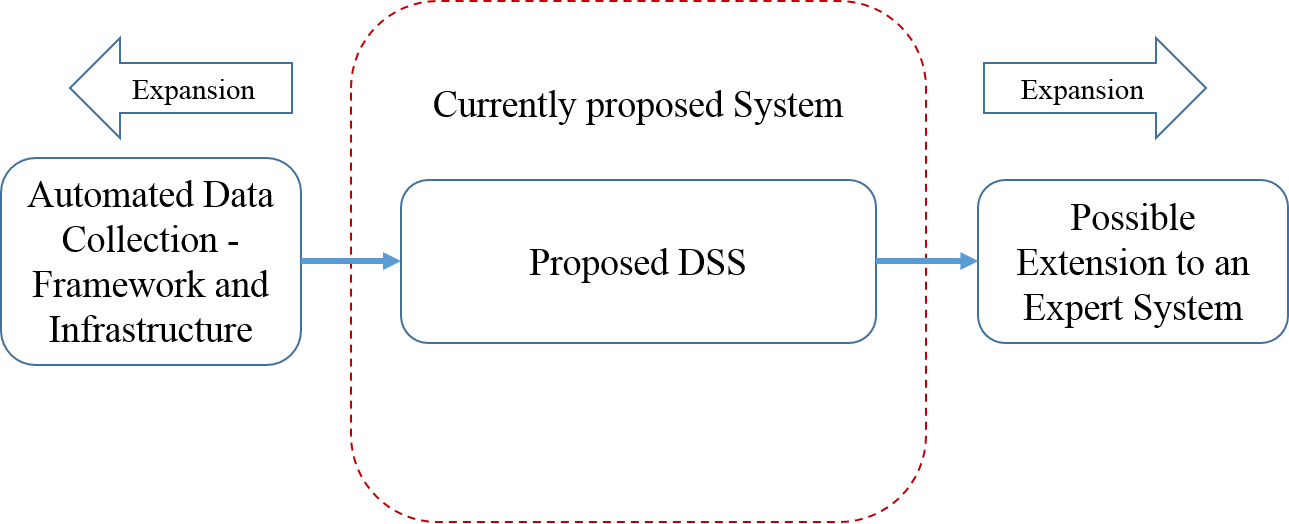
\includegraphics [scale=0.65] {futureWork}
\caption [Future Work and possible Expansion of Concept] {Future Work and possible Expansion of Concept}
\label {image-futureWork}
\end {figure}

\section{Conclusion}
\label{section-Conclusion}

\paragraph{} This research project looked at the public transportation problem in developing countries like Sri Lanka. The research commenced with the intention of looking into the problems that the Western Province Private Bus Service was facing and possibly providing solutions for them. Over the course of the project, the service and the prevalent system was analyzed and the requirements were gathered. Consequently a hypothesis was formed regarding the usage of a Decision Support System to alleviate the issues. A prototype was then built with the intention of gaining further insight into the requirements of the users and the concept of using a decision support system in the context of public transportation.

The main outcome of this research project was to identify and analyze the problems in the public transportation system in the western province. Testing the concept of using a decision support system within this domain was also an important outcome of this project. As this research project was carried out in an environment that is common to other developing nations, it can now be shown that a DSS with a similar architecture and concept would work in other developing countries as well. The main point of applying this \acrshort{dss} concept is the cost benefit. As this is an open-source project, it is greatly beneficial for government entities such as the \acrshort{wp} \acrshort{rpta}. Similarly, this same concept could be applied in other developing countries around the world.





